\documentclass[parskip=full,11pt]{scrartcl}
\usepackage[utf8]{inputenc}

\title{Simulator für wiederholte Spiele}
\author{Sebastian Feurer, Peter Koepernik, Luc Mercatoris,\\Christian Schorr, Pierre Toussing}

% section numbers in margins:
\renewcommand\sectionlinesformat[4]{\makebox[0pt][r]{#3}#4}

% header & footer
\usepackage{scrlayer-scrpage}
\lofoot{\today}
\refoot{\today}
\pagestyle{scrheadings}

\usepackage[sfdefault,light]{roboto}
\usepackage[T1]{fontenc}
\usepackage[german]{babel}
\usepackage[yyyymmdd]{datetime} % must be after babel
\renewcommand{\dateseparator}{-} % ISO8601 date format
\usepackage{hyperref}
\usepackage{amsmath} % for $\text{}$
\usepackage{amssymb}
\usepackage[nameinlink]{cleveref}
\crefname{figure}{Abb}{Abb}
\usepackage[section]{placeins}
\usepackage{xcolor}
\usepackage{graphicx}
\usepackage{subfig}
\hypersetup{
	pdftitle={Pflichtenheft},
	bookmarks=true,
}
\usepackage{csquotes}

\newcommand\urlpart[2]{$\underbrace{\text{\texttt{#1}}}_{\text{#2}}$}

\usepackage{pflichtenheft}

\def\adapt{Adaptionsschritt}
\def\adapts{Adaptionsschritte}

\def\segment{Segment}
\def\segments{Segmente}

\DeclareMathOperator*{\argmin}{arg\,min}

\begin{document}
\maketitle

\section{Einleitung}

Ziel dieses Projekts ist die Entwicklung einer Simulationsumgebung für wiederholte Spiele. Sie ist aus der Forschung motiviert und für den Einsatz in der Forschung ausgelegt. Die Simulationsumgebung wird verwendet, um das Entstehen von Gleichgewichtszuständen bei wiederholten Spielen mehrerer Agenten zu untersuchen. 

Es folgt eine Erläuterung des dem Simulator zugrundeliegenden Ablaufs. Dazu sei auch auf \cref{?} verwiesen.

Eine Simulation besteht aus mehreren Wiederholungen. Eine Wiederholung beginnt mit der Initialisierung der Agenten mit Strategien, Kapital und Gruppenzugehörigkeit. Anzahl der Agenten, Zuweisungsverfahren von Anfangsstrategien und Anfangskapital sowie Gruppeneinteilung werden vom Nutzer spezifiziert. Insbesondere legt der Nutzer die Menge aller möglichen Strategien fest. Danach folgen wiederholt \adapts, bis sich ein Gleichgewicht eingestellt hat oder eine konfigurierbare Höchstzahl an \adapts n erreicht ist. Ein \adapt\ besteht aus einer festen Zahl an Runden. In jeder Runde werden zunächst gemäß eines konfigurierbaren Algorithmus' Paare aus Agenten gebildet. Diese spielen dann gemäß ihrer aktuellen Strategie das dieser Simulation zugrundeliegende Stufenspiel. Nach Ablauf der Runden wird der Erfolg jedes Agenten in den zurückliegenden Runden quantifiziert und daraus eine Rangliste aller Agenten erstellt. Die Agenten passen nun ihre Strategien gemäß eines vom Nutzer spezifizierbaren Adaptionsmechanismus an. Ziel ist dabei nicht die Maximierung des Absolutkapitals, sondern eine möglichst hohe Position auf der Rangliste.

Nachdem alle Wiederholungen abgeschlossen sind, erfolgt die Ausgabe der Ergebnisse der einzelnen Wiederholungen. Wenn sich ein Gleichgewicht eingestellt hat, werden die Zahl der durchgeführten \adapts, die endgültigen Strategien und die endgültige Rangliste ausgegeben.

\pagebreak
\section{Kriterien}
% Diese Section sollte kurz und knapp "für Manager" sein
% und auf eine Seite passen.

\subsection{Muss}

\criterium{Starten einer Simulation}{crt:startsim}	

Der Nutzer kann eine Simulation starten, welche dann mit der aktuell gewählten Konfiguration durchgeführt wird.

\criterium{Ausgabe der Simulationsergebnisse}{crt:simresults_std}

Nach Durchführung einer Simulation wird für jede der Wiederholungen ausgegeben, ob sich ein Gleichgewicht eingestellt hat. Falls ja, werden die Zahl der durchgeführten \adapts, die endgültigen Strategien und die endgültige Rangliste ausgegeben.

\criterium{Abbrechen einer Simulation}{crt:cancelsim}

Der Nutzer kann eine laufende Simulation abbrechen.

\criterium{Anpassen von Simulationsparametern}{crt:simparam_std}

Der Nutzer hat die Möglichkeit, die folgenden Simulationsparameter festzulegen:
\begin{itemize} \itemsep -10pt
\item Anzahl der Agenten
\item zugrundeliegendes Stufenspiel
\item Anzahl verschiedener Gruppen und jeweils Anzahl zugehöriger Agenten
\item Zuweisungsverfahren für initiale Strategien
\item Menge aller möglichen Strategien
\item Zuweisungsverfahren für initiales Kapital
\item Algorithmus zur Bildung von Paaren beim Beginn einer Runde
\item Erfolgsquantifizierung zur Erstellung der Rangliste am Ende eines \adapt s
\item Adaptionsmechanismus, nach dem Agenten am Ende eines \adapt s ihre Strategien anpassen
\end{itemize}

\subsection{Kann}

\criteriumOptional{Detailliertere Ausgabe}{crt:simresults_add}
Nach Ablauf einer Simulation können für jede Wiederholung Rangliste und Strategien am Ende aller Adaptionsschritte eingesehen werden.

\criteriumOptional{Starten mehrerer Simulationen}{crt:multisim}
Es können mehrere Simulationen gleichzeitig laufen. Das Programm kann währenddessen unverändert verwendet werden und es wird eine Übersicht über alle gestarteten Simulationen und deren Ausführungsstatus angezeigt.

\criteriumOptional{Anpassen der Abbruchbedingungen}{crt:exitcondition}
Es können mehrere Kriterien für den Abbruch einer Wiederholung verwendet werden.

\criteriumOptional{Erweiterte Gruppenfunktionalität}{crt:groupfunc}
Gruppen und die Menge der gruppenlosen Agenten können jeweils in \segments\ unterteilt werden. Für jedes \segment\ können Zuweisungsverfahren für initiale Strategien und initiales Kapital separat festgelegt werden.

\criteriumOptional{Speichern und Laden von Konfigurationen}{crt:saveloadconfig}
Eine Konfiguration kann als Datei abgespeichert werden. Eine solche Konfigurationsdatei kann wiederum geladen werden.

\criteriumOptional{Erstellen eigener Strategien}{crt:createstrat}
Es können eigene Strategien erstellt werden.

\criteriumOptional{Erstellen eigener Stufenspiele}{crt:creategame}
Es können eigene Stufenspiele erstellt werden.

\criteriumOptional{Multikonfiguration}{crt:multikonf}
Der Nutzer kann eine Menge von Konfigurationen spezifizieren, in denen die Größe einer Gruppe oder die eines \segment s einer Gruppe eine festgelegte Folge von Werten durchläuft. Die so spezifizierten Simulationen werden gleichzeitig gestartet.

\subsection{Abgrenzung}

\criteriumNot{Kein alternativer Simulationsablauf}{crt:not_altsim}
Der zugrundeliegende Ablauf der Simulation, wie in der Einleitung erklärt, kann nicht verändert werden.

\criteriumNot{Keine komplexen Stufenspiele}{crt:not_complexgames}
Als Stufenspiele sind nur solche zugelassen, die sich als \(2 \times 2\) - Bimatrix mit konstanten Auszahlungen darstellen lassen.

\criteriumNot{Lokalisierung}{crt:local}
Die Anwendung soll nur in deutscher Sprache verfügbar sein.

\pagebreak

%%%%%%%%%%%
\section{Funktionale Anforderungen}

\functionality{Festlegung der Anzahl von Agenten}{fnc:agentcount}
\fulfills{crt:simparam_std}
Der Nutzer hat die Möglichkeit, die Anzahl von Agenten in einem Simulationsdurchlauf festzulegen.

Die gewünschte Zahl kann im Konfigurationsfenster über einen Slider eingestellt werden. Zugelassen sind gerade Zahlen zwischen \(2\) und \(10.000\). Im Textfeld rechts des Sliders wird der eingestellte Zahlenwert angezeigt. Das Festlegen des Wertes ist auch durch direkte Eingabe in das Textfeld möglich, der Slider wird dann automatisch auf die entsprechende Position gesetzt. Voreingestellt sind \(100\) Agenten.

\functionality{Festlegung des Stufenspiels}{fnc:selectgame}
\fulfills{crt:simparam_std}
Der Nutzer kann das einem Simulationsdurchlauf zugrundeliegende Stufenspiel festlegen.

Dazu befindet sich im Konfigurationsfenster ein Dropdown-Menü. Wird dieses angeklickt, so kann ein Stufenspiel aus einer Liste aller im System hinterlegten Stufenspiele ausgewählt werden. Rechts des Dropdown-Menüs wird eine kurze Beschreibung des aktuell eingestellten Stufenspiels angezeigt (siehe \cref{?}).

Abgesehen von selbst erstellten Stufenspielen sind folgende Stufenspiele im System hinterlegt:
\begin{itemize} \itemsep -10pt
\item Gefangenendilemma
\item Hirschjagd
\item Feiglingsspiel
\item Kampf der Geschlechter
\item Vertrauensspiel
\item Elfmeterschießen
\end{itemize}
Voreingestellt ist das Gefangenendilemma.

\functionality{Festlegung der Anzahl von Runden}{fnc:rounds}
\fulfills{crt:simparam_std}
Der Nutzer hat die Möglichkeit, die Anzahl pro \adapt\ durchgeführter Runden festzulegen.

Wie die Anzahl von Agenten kann die Anzahl von Runden im Konfigurationsfenster mittels Slider bzw. Textfeld eingestellt werden. Zugelassen sind natürliche Zahlen zwischen \(50\) und \(1000\). Voreingestellt sind \(100\) Runden.

\functionality{Festlegung der Anzahl von Wiederholungen}{fnc:repeats}
\fulfills{crt:simparam_std}
Der Nutzer hat die Möglichkeit, die Anzahl pro Simulation durchgeführter Wiederholungen festzulegen.

Wie die Anzahl von Agenten kann die Anzahl von Wiederholungen im Konfigurationsfenster mittels Slider bzw. Textfeld eingegeben werden. Zugelassen sind natürliche Zahlen zwischen \(1\) und \(10\). Voreingestellt sind \(5\) Wiederholungen.

\functionality{Festlegung der Menge aller möglichen Strategien}{fnc:stratset}
\fulfills{crt:simparam_std}
Der Nutzer kann bei der Konfiguration einer Simulation die Menge aller Strategien festlegen, die in dieser Simulation von Agenten verwendet werden können.

Dazu befindet sich im Konfigurationsfenster ein 'Strategie hinzufügen'-Knopf. Darunter befindet sich eine Liste aller bereits hinzugefügten Strategien (siehe \cref{?}). Bei Betätigen des 'Strategie hinzufügen'-Knopfes öffnet sich ein Fenster mit einer Liste aller im System hinterlegten Strategien. Mittels üblicher \textsf{CTRL}- und \textsf{SHIFT}-Klick-Funktionalität können eine oder mehrere Strategien ausgewählt werden. Bereits hinzugefügte Strategien sind ausgegraut und können nicht ausgewählt werden (siehe \cref{?}). Beim Betätigen des 'Bestätigen'-Knopfes wird das Fenster geschlossen und alle ausgewählten Strategien werden zu der Liste hinzugefügt. Beim Betätigen des 'Abbrechen'-Knopfes wird das Fenster geschlossen und keine Strategien werden hinzugefügt. Unter der Liste der hinzugefügten Strategien befindet sich eine Checkbox mit der Bezeichnung 'gemischte Strategien'. Ist diese aktiviert, so können Agenten im Laufe der Simulation gemischte Strategien entwickeln. Ist die Checkbox deaktiviert, werden nur reine Strategien verwendet.

In der Liste der ausgewählten Strategien befindet sich neben jeder Strategie ein '\(\circleddash\)'-Knopf. Wird dieser betätigt, wird die Strategie aus der Liste entfernt.

Abgesehen von selbst erstellten Strategien sind folgende Strategien im System hinterlegt:
\begin{itemize} \itemsep -10pt
\item Tit-for-tat
\item Grim
\item Kooperation mit Agenten mit ähnlichem Absolutkapital\footnote{Das Absolutkapital zweier Agenten ist ähnlich, genau dann wenn sich der Rang der Agenten, aufgelistet nach Absolutkapital, höchstens um \(20\%\) der Gesamtzahl aller Agenten unterscheidet.}, ansonsten keine Kooperation
\item Tit-for-tat mit Agenten mit ähnlichem Absolutkapital, ansonsten keine Kooperation
\item Keine Kooperation mit Agenten mit höherem Absolutkapital, ansonsten tit-for-tat
\item Keine Kooperation mit Agenten mit niedrigerem Absolutkapital, ansonsten tit-for-tat
\item Kooperation mit Agenten derselben Gruppenzugehörigkeit, ansonsten keine Kooperation
\item Tit-for-tat mit Agenten derselben Gruppenzugehörigkeit, ansonsten keine Kooperation
\item Immer Kooperation
\item Nie Kooperation
\end{itemize}
Voreingestellt sind Tit-for-tat, Grim und \glqq Immer Kooperation\grqq.

\functionality{Konfiguration von Anzahl und Größe der Gruppen}{fnc:groups}
\fulfills{crt:simparam_std}
Der Nutzer hat die Möglichkeit, die Anzahl verschiedener Gruppen in einem Simulationsdurchlauf festzulegen. Weiterhin kann er angeben, wie viele Agenten den einzelnen Gruppen und wie viele Agenten keiner Gruppe zugehörig sind.

Dazu muss im Konfigurationsfenster der Abschnitt 'Gruppeneinstellungen' durch Drücken des Knopfes am linken Rand des entsprechend benannten Separators ausgeklappt werden (siehe \cref[{}). Voreingestellt sind null Gruppen. Eine neue Gruppe kann durch Betätigen des 'Gruppe hinzufügen'-Knopfes hinzugefügt werden (siehe \cref{?}). Jeder Gruppe wird bei Erstellung eine zufällige, unter allen Gruppen eindeutige Farbe zugeordnet. Ist die maximale Anzahl von fünf Gruppen erreicht, ist der 'Gruppe hinzufügen'-Knopf ausgegraut und kann nicht mehr betätigt werden.

Eine Gruppe wird beim Hinzufügen mit null Mitgliedern initialisiert. Die Anzahl der Mitglieder einer Gruppe kann über den Multislider links des 'Gruppe hinzufügen'-Knopfes verändert werden. Für jede Gruppe befindet sich ein entsprechend gefärbter Schiebe-Knopf auf dem Multislider. Der Slider-Abschnitt links des Knopfes wird ebenfalls mit der Gruppenfarbe gefärbt. Die relative Größe jeder Gruppe entspricht genau der relativen Größe des entsprechend gefärbten Abschnitts auf dem Slider. Der rechtsgelegenste Abschnitt ist weiß gefärbt und gibt die Anzahl der gruppenlosen Agenten an. Über jedem Abschnitt wird die Zahl von Agenten angezeigt, die diesem Abschnitt angehören (siehe \cref{?}). Wird durch Verschieben eines Sliders die Größe einer Gruppe verändert, so ändern sich die Größen anderer Gruppen nicht. Beim Vergrößern einer Gruppe sinkt also die Zahl der gruppenlosen Agenten, beim Verkleinern einer Gruppe vergrößert sie sich. Folglich kann keine Gruppe vergrößert werden, wenn bereits alle Agenten einer Gruppe angehören.

Die Abschnitte des Sliders fungieren als Tab-Control. Unterhalb des Sliders befindet sich ein Abschnitt zur Konfiguration der aktuell per Tab-Control ausgewählten Gruppe bzw. der gruppenlosen Agenten (siehe \cref{?}). Im Konfigurationsabschnitt einer Gruppe befindet sich ein 'Gruppe löschen'-Knopf. Wird dieser betätigt, öffnet sich ein Bestätigungs-Dialog (siehe \cref{?}). Wird in diesem auf 'Abbrechen' gedrückt, schließt sich der Dialog und die Konfiguration bleibt unverändert. Wird auf 'Bestätigen' gedrückt, schließt sich der Dialog und die Gruppe wird gelöscht. Das Tab-Control wechselt zu den gruppenlosen Agenten und die Mitglieder der gelöschten Gruppe werden gruppenlos.

\functionality{Einteilung von Gruppen in \segments}{fnc:segments}
\fulfills{crt:groupfunc}
Der Nutzer kann jede Gruppe und die Menge der gruppenlosen Agenten in ein bis fünf \segments\ unterteilen. Für jedes \segment\ können die Zuweisungsverfahren für initiale Strategien und initiales Kapital separat konfiguriert werden.

Die Unterteilung erfolgt im Konfigurationsabschnitt einer Gruppe bzw. der gruppenlosen Agenten. Am oberen Ende des Abschnittes befindet sich eine Überschrift '\segment einstellungen', darunter ein Multislider und ein '\segment\ hinzufügen'-Knopf (siehe \cref{?}). Voreingestellt ist ein Segment. Ein neues Segment kann durch Betätigen des '\segment\ hinzufügen'-Knopfes hinzugefügt werden. Ist die maximale Anzahl von fünf \segments n erreicht, ist der '\segment\ hinzufügen'-Knopf ausgegraut und kann nicht mehr betätigt werden. Für jedes hinzugefügte Segment erscheint auf dem Multislider ein Schiebe-Knopf. Wie bei den Gruppeneinstellungen entspricht jeder Abschnitt auf dem Slider einem \segment. Durch Verschieben der Schiebe-Knöpfe kann so die Größe der \segments\ verändert werden. Die Abschnitte fungieren als Tab-Control, und unter dem Slider befindet sich ein Konfigurationsabschnitt für das aktuell ausgewählte \segment. Der Konfigurationsabschnitt enthält die Einstellungen für das Zuweisungsverfahren für initiale Strategien und initiales Kapital.

Am unteren Ende des Konfigurationsabschnittes eines \segment s befindet sich ein '\segment\ löschen'-Knopf. Betätigen des Knopfes öffnet einen Bestätigungs-Dialog. Wird in diesem auf 'Abbrechen' gedrückt, so schließt sich der Dialog und die Konfiguration bleibt unverändert. Wird in dem Dialog auf 'Bestätigen' gedrückt, so schließt sich der Dialog und das \segment\ wird entfernt. Gibt es nur noch ein \segment, so ist der '\segment\ löschen'-Knopf ausgegraut und kann nicht betätigt werden.

\functionality{Konfiguration des Zuweisungsverfahrens für initiale Strategien}{fnc:initialstrat}
\fulfills{crt:simparam_std}
\fulfills{crt:groupfunc}
Der Nutzer kann das Zuweisungsverfahren für die initialen Strategien der Agenten beim Beginn einer Wiederholung einstellen. Diese Einstellung findet für jedes \segment\ einer Gruppe und für jedes \segment\ der gruppenlosen Agenten separat statt.

Die Einstellung erfolgt in dem Konfigurationsabschnitt eines \segment s. Dort befindet sich ein mit 'Initiale Strategien' beschrifteter Unterabschnitt. In diesem befinden sich zwei nebeneinander angeordnete List-Boxen (siehe \cref{?}). Die Linke ist beschriftet mit 'Alle Strategien', die Rechte mit 'Gewählte Strategien'. In der linken Box sind alle Strategien aufgelistet, die der Nutzer für diese Simulation zugelassen hat. Die rechte Box ist zunächst leer. Per üblicher \textsf{CTRL}- und \textsf{SHIFT}-Klick-Funktionalität können eine oder mehrere Strategien in der linken Box ausgewählt werden. Betätigen des 'Hinzufügen'-Knopfes zwischen den beiden Boxen entfernt alle ausgewählten Strategien aus der linken Box und fügt sie in die rechte Box ein. Analog können Strategien in der rechten Box ausgewählt und mittels Betätigen des 'Entfernen'-Knopfes aus der rechten Box entfernt und in die Linke wieder eingefügt werden.

Zu Beginn jeder Wiederholung in einer so konfigurierten Simulation wird jedem Agent aus dem aktuell konfigurierten \segment\ zufällig eine Strategie aus der Liste der gewählten Strategien zugeordnet. Ist diese Liste leer, werden den Agenten zufällige Strategien aus der Menge aller zugelassenen Strategien zugeordnet. Insbesondere werden Agenten immer mit reinen Strategien initialisiert.

\functionality{Konfiguration des Zuweisungsverfahrens für initiales Kapital}{fnc:initialcap}
\fulfills{crt:simparam_std}
\fulfills{crt:groupfunc}
Der Nutzer kann das Zuweisungsverfahren für das initiale Kapital der Agenten beim Beginn einer Wiederholung einstellen. Diese Einstellung findet für jedes \segment\ einer Gruppe und für jedes \segment\ der gruppenlosen Agenten separat statt.

Die Einstellung erfolgt in dem Konfigurationsabschnitt eines \segment s. Dort befindet sich ein mit 'Initiales Kapital' beschrifteter Unterabschnitt (siehe \cref{?}). Mittels Radiobuttons kann eine der folgenden Wahrscheinlichkeitsverteilungen gewählt werden:
\begin{itemize}
\item Gleichverteilung
\item Binomialverteilung
\item Poissonverteilung
\item festes Ergebnis
\end{itemize}
Unter den Radiobuttons befinden sich Eingabemöglichkeiten zur Parametrisierung der aktuell gewählten Verteilung, eine kurze Beschreibung und ein Graph der Verteilung. Voreingestellt ist das feste Ergebnis \(0\), also kein Anfangskapital.

Für die Gleichverteilung müssen die beiden Intervallgrenzen \(a,b \in \mathbb{N}_0, \ a < b\) in Textfeldern angegeben werden. Voreingestellt ist \(a = 0, b = 100\) (siehe \cref{?}).

Bei der Binomialverteilung müssen die Intervallgrenzen \(a,b \in \mathbb{N}_0, \ a < b\) in Textfeldern und der Parameter \(p \in (0,1)\) mittels Slider angegeben werden. Voreingestellt ist \(a = 0, b = 100, p = 0.5\) (siehe \cref{?}).

Bei der Poisson-Verteilung muss der Parameter \(\lambda \in \mathbb{N}_0\) in einem Textfeld angegeben werden. Voreingestellt ist \(\lambda = 50\) (siehe \cref{?}).

Beim festen Ergebnis muss der Parameter \(a \in \mathbb{N}_0\), der das feste Ergebnis angibt, in einem Textfeld angegeben werden. Voreingestellt ist \(a = 0\) (siehe \cref{?}).

Bei fehlerhafter Eingabe eines Parameters wird die Eingabe auf den nächsten zugelassenen Wert abgeändert.

Zu Beginn jeder Wiederholung in einer so konfigurierten Simulation wird jedem Agent aus dem aktuell konfigurierten \segment\ ein zufälliger Betrag als initiales Kapital zugewiesen, gezogen aus der eingestellten Wahrscheinlichkeitsverteilung.

\functionality{Festlegen des Algorithmus zur Paarbildung}{fnc:algopaar}
\fulfills{crt:simparam_std}

Im Konfigurationsfenster kann der Nutzer durch einen Klick auf \enquote{Erweiterte Einstellungen} das \enquote{Paarbildungs}-DropDown-Menü anzeigen lassen. Durch Betätigen des \enquote{Paarbildungs}-DropDown-Menü werden ihm die Möglichkeiten:\begin{itemize} \itemsep -10pt
\item zufällige Paarbildung
\newline Erklärung: Jedem Agenten wird ein zufälliger Spielpartner zugeordnet.
\item unter Berücksichtigung der Kooperationswahrscheinlichkeit
\newline Erklärung: Jedem Agenten wird ein Spieler mit einer hohen Wahrscheinlichkeit das er kooperiert (beruhend auf vergangenen Spielrunden) zugeordnet.
\item unter Berücksichtigung der Gruppe
\newline Erklärung: Jedem Agenten wird ein Mitglied seiner Gruppe zugeordnet, falls dies möglich ist.
\end{itemize}angezeigt. Durch Klicken auf zufällige Paarbildung, unter Berücksichtigung der Kooperationswahrscheinlichkeit oder unter Berücksichtigung der Gruppe legt der Nutzer den Algorithmus zur Paarbildung fest.

\functionality{Festlegen der Erfolgsquantifizierung}{fnc:erfolg}
\fulfills{crt:simparam_std}

Im Konfigurationsfenster kann der Nutzer durch einen Klick auf \enquote{Erweiterte Einstellungen} das \enquote{Erfolgsquantifizierungs}-DropDown-Menü anzeigen lassen. Durch Betätigen des \enquote{Erfolgsquantifizierungs}-DropDown-Menü werden ihm die Möglichkeiten:\begin{itemize} \itemsep -10pt
\item durchschnittliche Absolutauszahlung
\newline Erklärung: Das arithmetische Mittel der Auszahlungen über alle bisherigen Runden.
\item gleitender Durschnitt
\newline Erklärung: Nach dem Prinzip des SMA(Simple Moving Average) wird das arithmetische Mittel über die Zeitspanne der letzen X Runden gebildet. X ist hierbei ein prozentualer Anteil von der Gesamtzahl der bisher gespielten Runden.
\end{itemize}angezeigt. Durch Klicken auf Absolutauszahlung beziehungsweise gleitender Durchschnitt legt er diese als Erfolgsquantifizierung fest.

\functionality{Festlegen des Adaptionsmechanismus}{fnc:algoadapt}
\fulfills{crt:simparam_std}
Der Nutzer hat die Möglichkeit, den Mechanismus festzulegen, mit dem die Agenten am Ende eines \adapt s ihre Strategien anpassen.

Dazu befindet sich im Konfigurationsfenster im Abschnitt \glqq Erweiterte Einstellungen\grqq\ ein Dropdown-Menü mit der Bezeichnung \glqq Adaptionsmechanismus\grqq. Über dieses kann einer der folgenden Mechanismen ausgewählt werden:

\textbf{Replicator Dynamic:}
Dieser Mechanismus hat zwei Konfigurationsparameter: Einen Wert \(\alpha \in (0,1)\), und einen Wert \(\beta \in (0,\frac{1}{N-1})\), wobei \(N\) die Anzahl der Agenten bezeichnet. Für jeden Agenten A passiert dann nach der Erstellung der Rangliste am Ende eines \adapt s folgendes: Mit der Wahrscheinlichkeit \(1 - \alpha\) ändert A seine Strategie nicht. Andernfalls wird ein ein anderer Agent B zufällig gewählt. \(\Delta r\) bezeichne nun die Differenz der Ränge von A und B. Ist \(\Delta r < 0\), so ändert A seine Strategie nicht. Ist \(\Delta r > 0\) und sind nur reine Strategien zugelassen, so übernimmt Agent A mit Wahrscheinlichkeit \(\delta := \beta \cdot \Delta r \in (0,1)\) die Strategie von Agent B. Sind gemischte Strategien erlaubt, so wird stattdessen mit Parameter \(\delta\) zwischen Strategie von A und Strategie von B linear interpoliert und das Ergebnis auf die in der Summennorm nächstmögliche gültige Strategie gerundet, d.h.
\[
\omega_\text{A}^\text{(neu)} = \underset{\omega \in \Omega}{\operatorname{arg min}} \|\omega - \omega^*\|_1 \text{  mit  } \omega^* = \omega_\text{A} + \delta \cdot (\omega_\text{B} - \omega_\text{A}),
\]
wobei \(\Omega = \{\omega \in \{0,\frac{1}{10},...,1\}^n | \sum_{i=1}^n \omega_i = 1\}\) die Menge aller gültigen gemischten Strategien, \(n\) die Anzahl von in diesem Simulationslauf möglichen Strategien und \(\omega_\text{A}\), \(\omega_\text{B}\) die aktuellen Strategien von A und B bezeichnen\footnote{\(\|\cdot\|_1 : \mathbb{R}^n \rightarrow [0,\infty), \ x = (x_i)_{i=1}^n \mapsto \sum_{i=1}^n |x_i|\) bezeichnet die Summennorm auf \(\mathbb{R}^n\).}. Voreinstellungen für die Parameter sind \(\alpha = 0.5\) und \(\beta = \frac{0.5}{N - 1}\).

\textbf{Preferential Adaption:}
Dieser Mechanismus hat zwei Konfigurationsparameter: Einen Wert \(\alpha \in (0,1)\), und einen Wert \(\beta \in (0,\frac{1}{N-1})\), wobei \(N\) die Anzahl der Agenten bezeichnet. Es sei nun \(p_{ij}\) für \(i,j \in \{1,...,N\}, i \neq j\) die Wahrscheinlichkeit, dass der \(i\)-te Agent nach aktueller Strategie mit dem \(j\)-ten Agenten kooperieren würde\footnote{Sind nur reine Strategien zugelassen, ist also \(p_{ij} \in \{0,1\} \forall i,j \in \{1,...,N\}, i \neq j\)}. Für den \(i\)-ten Agenten A passiert dann nach der Erstellung der Rangliste am Ende eines \adapt s folgendes: Mit der Wahrscheinlichkeit \(1 - \alpha\) ändert A seine Strategie nicht. Andernfalls wird ein anderer Agent B zufällig gewählt. Die Wahrscheinlichkeit \(p_j\), dabei den \(j\)-ten Agenten zu wählen, beträgt
\[
p_j = \frac{p_{ij}}{\sum_{l \neq i} p_{il}}.
\]
Ist nun der \(j\)-te Agent B gewählt, so bezeichne \(\Delta r\) die Differenz der Ränge von A und B. Ist \(\Delta r < 0\), so ändert A seine Strategie nicht. Ist \(\Delta r > 0\), so sei \(\delta := p_{ij} \cdot \beta \cdot \Delta r\). Wie bei \glqq Replicator Dynamic\grqq\ wird nun die Strategie von B mit Wahrscheinlichkeit \(\delta\) übernommen bzw. linear interpoliert. Voreingestellt sind \(\alpha = 0.5\) und \(\beta = \frac{0.5}{N - 1}\).

Unter dem Dropdown-Menü befinden sich Slider und Textfelder zur Eingabe der für den ausgewählten Mechanismus notwendigen Parameter. Voreingestellt ist \glqq Replicator Dynamic\grqq.

\functionality{Festlegen der Abbruchbedingungen}{fnc:exitcondition}
\fulfills{crt:exitcondition}
Der Nutzer hat die Möglichkeit, die Abbruchbedingungen für Wiederholungen festzulegen. Einerseits kann er ein Gleichgewichtskriterium festlegen. Andererseits kann er eine maximale Anzahl durchzuführender \adapts\ angeben. Wird in einer Wiederholung im so konfigurierten Simulationslauf ein Gleichgewicht oder die festgelegte Schranke an \adapts n erreicht, so wird die Wiederholung beendet und gegebenenfalls die nächste gestartet.

Zur Einstellung befindet sich im Konfigurationsfenster im Abschnitt \glqq Erweiterte Einstellungen\grqq\ ein Dropdown-Menü mit der Bezeichnung \glqq Abbruchbedingung\grqq. Über dieses kann eines der folgenden Gleichgewichtskriterien ausgewählt werden:

\textbf{Gleichgewicht nach Strategien:}
Dieses Kriterium hat zwei freie Konfigurationsparameter \(\alpha \in (0,1)\) und \(G \in \{10,...,200\}\). Für zwei aufeinanderfolgende \adapts\ wird auf folgende Art ein Maß \(\Delta_\text{S}\) für die Änderungen in den Strategien der Agenten berechnet: Sind nur reine Strategien zugelassen, ist \(\Delta_\text{S}\)  die Zahl aller Agenten, die ihre Strategie geändert haben. Sind gemischte Strategien zugelassen, so bezeichne \(\omega_i\) bzw. \(\omega_i'\) die Strategie des \(i\)-ten Agenten in den beiden \adapts n (\(i \in \{1,...,N\}\) mit der Anzahl \(N\) aller Agenten). Dann ist
\[
\Delta_\text{S} :=\frac 12 \sum_{i=1}^N \|\omega_i - \omega_i'\|_1.
\]
Ist nun \(\Delta_\text{S} < \alpha \cdot N\) in \(G\) aufeinanderfolgenden \adapts n, so ist ein Gleichgewicht nach Strategien erreicht.

\textbf{Gleichgewicht nach Rang:}
Dieses Kriterium hat zwei freie Konfigurationsparameter \(\alpha \in (0,1)\) und \(G \in \{10,...,200\}\). Für zwei aufeinanderfolgende \adapts\ bezeichne \(r_i\) bzw. \(r_i'\) den Rang des \(i\)-ten Agenten in den beiden \adapts n (\(i \in \{1,...,N\}\) mit der Anzahl \(N\) aller Agenten). Dann wird gemäß
\[
\Delta_\text{R} := \sum_{i=1}^N |r_i - r_i'|,
\]
ein Maß für die Änderungen in der Rangliste zwischen den aufeinanderfolgenden \adapts n berechnet. Ist nun \(\Delta_\text{R} < \alpha \cdot \frac{N^2}{2}\) in \(G\) aufeinanderfolgenden \adapts n, so ist ein Gleichgewicht nach Rang erreicht.

Unter dem Dropdown-Menü befinden sich Slider und Textfelder zur Eingabe der für das ausgewählte Gleichgewichtskriterium notwendigen Parameter. Voreingestellt ist \glqq Gleichgewicht nach Strategien\grqq\ mit \(\alpha = 0.1\) und \(G = 100\). Ebenfalls unter dem Dropdown-Menü befindet sich ein Slider zur Einstellung der maximalen Anzahl durchzuführender \adapts\. Möglich sin natürliche Zahlen zwischen \(100\) und \(10.000\). Voreingestellt sind \(3.000\).

\functionality{Multikonfiguration von Gruppen}{fnc:multikonfgr}
\fulfills{crt:multikonf}
Beträgt die Anzahl von Gruppen in einer Konfiguration genau Eins, kann die Gruppen - Multikonfiguration aktiviert werden. Diese ermöglicht das gleichzeitige Starten mehrerer Simulationen, in denen die Gruppengröße alle Werte in einem spezifizierbaren Intervall mit einer spezifizierbaren Schrittgröße einmal annimmt. Dazu muss eine Checkbox mit der Bezeichnung \glqq Multikonfiguration\grqq\ unter dem Slider zur Einstellung der Gruppengröße aktiviert werden. Daraufhin werden der Slider zur Einstellung der Gruppengrößen und der \glqq Gruppe hinzufügen\grqq -Knopf ausgegraut und können nicht mehr bedient werden (siehe \cref{?}). Im Abschnitt \glqq Erweiterte Einstellungen\grqq\ unter den Gruppeneinstellungen befindet sich ein mit \glqq Multikonfiguration\grqq\ beschrifteter Unterabschnitt (siehe \cref{?}). Mit einem Range-Slider kann dort ein Teilintervall von \([0,100]\%\) eingestellt werden, wobei für linke und rechte Grenze nur Vielfache von \(10\%\) möglich sind. Über einen Slider kann die Schrittgröße eingestellt werden, wobei nur Vielfache von \(5\%\) zwischen \(5\%\) und der Breite des eingestellten Intervalls möglich sind.

Beim Starten einer so konfigurierten Simulation wird für jeden Wert im spezifizierten Intervall gemäß der spezifizierten Schrittgröße eine Simulation gestartet, in der die Größe der Gruppe einen entsprechenden Anteil an der Zahl aller Agenten hat. Die restlichen Konfigurationsparameter bleiben gleich.

Ist die aktuell eingestellte Anzahl von Gruppen nicht Eins oder wurde für eine Gruppe bereits die \segment -Multikonfiguration aktiviert, so kann die Gruppen-Multikonfiguration nicht aktiviert werden.

\functionality{Multikonfiguration von \segments n}{fnc:multikonfseg}
\fulfills{crt:multikonf}
Besteht eine Gruppe aus genau zwei \segments n, so kann für diese Gruppe die \segment -Multikonfiguration aktiviert werden. Diese ermöglicht das gleichzeitige Starten mehrerer Simulationen, in denen die \segment größe des ersten \segment s der so konfigurierten Gruppe alle Werte in einem spezifizierbaren Intervall mit einer spezifizierbaren Schrittgröße einmal annimmt. Dazu muss eine Checkbox mit der Bezeichnung \glqq Multikonfiguration\grqq\ unter dem Slider zur Einstellung der \segment größen aktiviert werden. Daraufhin werden der Slider zur Einstellung der \segment größen und der \glqq \segment\ hinzufügen\grqq -Knopf ausgegraut und können nicht mehr bedient werden (siehe \cref{?}). Wie bei der Gruppen-Multikonfiguration können nun im Unterabschnitt \glqq Multikonfiguration\grqq\ im Abschnitt \glqq Erweiterte Einstellungen\grqq\ Intervall und Schrittgröße eingegeben werden.

Beim Starten einer so konfigurierten Simulation wird für jeden Wert im spezifizierten Intervall gemäß der spezifizierten Schrittgröße eine Simulation gestartet, in der das erste \segment\ der Gruppe entsprechend groß ist und das zweite \segment\ den Rest der Gruppe einnimmt. Die restlichen Konfigurationsparameter bleiben gleich.

Ist die aktuell eingestellte Zahl von \segments n einer Gruppe nicht Zwei oder wurde die Gruppen-Multikonfiguration oder die \segment -Multikonfiguration für eine andere Gruppe bereits aktiviert, so kann die \segment -Multikonfiguration für diese Gruppe nicht aktiviert werden.

\functionality{Simulation starten}{fnc:simstart}
\fulfills{crt:startsim}
\fulfills{crt:multisim}
Der Nutzer kann eine Simulation starten, in dem er den \glqq Play\grqq -Knopf im oberen rechten Bereich des Start-Fensters betätigt (siehe \cref{?}). Das Programm führt dann den in der Einleitung beschriebenen Simulationsablauf mit den in der aktuellen Konfiguration festgelegten Parametern durch. Das Programm kann während dem Simulationsdurchlauf weiterhin unverändert verwendet werden. Insbesondere können weitere Simulationen gestartet werden. Ist die maximale Anzahl von \(20\) laufenden Simulationen erreicht, ist der \glqq Play\grqq -Knopf ausgegraut und kann nicht mehr betätigt werden.

\functionality{Anzeige laufender und abgeschlossener Simulationen}{fnc:anzeigesim}
\fulfills{crt:multisim}
Im Startfenster wird eine Liste aller gestarteten Simulationen angezeigt (siehe \cref{?}). Jeder Listeneintrag beinhaltet den Ausführungsstatus der zugehörigen Simulation. Eine Menge von durch Multikonfiguration gestarteten Simulationen nimmt nur einen Listeneintrag ein. Dieser gibt Auskunft über den Ausführungsstatus aller zugehörigen Simulationen.

Ist eine Simulation abgeschlossen, so fungiert der zugehörige Listeneintrag als Knopf. Wird dieser betätigt, so werden rechts der Liste Informationen über die Ergebnisse der Simulation angezeigt.

\functionality{Abbrechen einer Simulation}{fnc:cancelsim}
\fulfills{crt:cancelsim}
Eine noch nicht abgeschlossene Simulation kann abgebrochen werden. Dazu muss der Mauszeiger über den entsprechenden Listeneintrag im Startfenster bewegt werden. Wird der dann erscheinende mit \glqq X\grqq\ beschriftete Knopf betätigt, so wird die Simulation abgebrochen und aus der Liste entfernt. Der Abbruch einer Menge von durch Multikonfiguration gestarteten Simulationen führt zum Abbruch aller zugehörigen Simulationen und zum Löschen der Ergebnisse der möglicherweise bereits abgeschlossenen Simulationen.

\functionality{Stufenspiel erstellen}{fnc:createNewGame}
\fulfills{crt:creategame}

Der Nutzer kann im Konfigurations- und Hauptfenster in der Menüleiste den Reiter Erweiterungen auswählen und Stufenspiel erstellen anklicken. Alternativ kann er im Konfigurationsfenster den \enquote{Stufenspiel erstellen}-Button in der Toolbar anklicken. Daraufhin öffnet sich das Stufenspielerstellenfenster \textbf{(siehe Bild)}. Im Textfeld hinter der Schrift Name: kann der Name des Stufenspiels eingetragen werden. Der Nutzer kann in die Bimatrix die jeweiligen Auszahlungen schreiben. Es sind die Auszahlungen bei nicht-Kooperation beider Spieler, Kooperation beider Spieler, nicht-Kooperation von Spieler 1 und Kooperation von Spieler 2 und Kooperation von Spieler 1 und nicht-Kooperation von Spieler 2 jeweils mit der Auszahlung für Spieler 1 und der Auszahlung von Spieler 2 zu füllen. Im Textbereich Beschreibung kann eine Beschreibung des Spiels Stufenspiel eingegeben werden. Durch Betätigen des \enquote{Speichern}-Buttons kann das Stufenspiel gespeichert werden. Das Stufenspiel erscheint dann in der Stufenspielauswahl des Konfigurationsfensters. Alternativ kann der Vorgang über den \enquote{Abbrechen}-Button abgebrochen werden.

\functionality{Konfiguration bearbeiten}{fnc:editConfig}
\fulfills{crt:simparam_std}

Der Nutzer kann im Hauptfenster den \enquote{Konfiguration bearbeiten}-Button \textbf{(siehe Bild)} auswählen und damit das Konfigurationsfenster öffnen. Dies ermöglicht ihm die aktuelle Konfiguration zu ändern.

\functionality{Konfiguration laden}{fnc:loadConfig}
\fulfills{crt:saveloadconfig}

Der Nutzer kann im Konfigurationsfenster und im Hauptfenster auf die Menüleiste \textbf{(siehe Bild)} zugreifen. Durch auswählen des Reiters Datei und anschließendem Klick auf Konfiguration laden öffnet sich ein neues Fenster(Datei-öffnen Dialog). Alternativ kann dieses Fenster auch im Konfigurationsfenster durch einen Klick auf den \enquote{Konfiguration laden}-Button in der Toolbar \textbf{(siehe Bild)} geöffnet werden. In dem neu geöffneten Fenster wird das Verzeichnis, in dem die Konfigurationen standardmäßig abgespeichert werden, angezeigt. Die Konfigurationen können mit einem Klick auf diese und anschließendem Klick auf den \enquote{Laden}-Button geladen werden. Daraufhin schließt sich das Fenster und die geladenen Konfigurationsdaten erscheinen im geöffneten Fenster. Alternativ kann man den Vorgang mit einem Klick auf den \enquote{Abbrechen}-Button abbrechen und das Fenster schließt sich.

\functionality{Konfiguration speichern}{fnc:saveConfig}
\fulfills{crt:saveloadconfig}

Der Nutzer kann im Konfigurationsfenster und im Hauptfenster auf die Menüleiste \textbf{(siehe Bild)} zugreifen. Durch auswählen des Reiters Datei und anschließendem Klick auf Konfiguration speichern öffnet sich ein neues Fenster(Datei- speichern Dialog). Alternativ kann dieses Fenster auch im Konfigurationsfenster durch einen Klick auf den \enquote{Konfiguration speichern}-Button in der Toolbar \textbf{(siehe Bild)} geöffnet werden. In dem neu geöffnete Fenster zeigt das Verzeichnis in dem die Konfigurationen gespeichert werden. Nun kann der Nutzer den Namen seiner Konfiguration in das Textfeld Dateiname eingeben. Die Konfiguration kann mit einem Klick auf den \enquote{Speichern}-Button gespeichert werden. Daraufhin schließt sich das Fenster. Alternativ kann man den Vorgang mit einem Klick auf den \enquote{Abbrechen}-Button abbrechen und das Fenster schließt sich.

%%%%%%%%%%%
\section{Nicht-Funktionale Anforderungen}

\nonFunctionality{Design}{nfc:design}

Das Design soll modern und seriös wirken. Es soll schnörkellos sein und sich auf die für die Wissenschaft relevanten Dinge fokussieren.

\nonFunctionality{Erweiterbarkeit}{nfc:extensibility}

Das Produkt muss dahingehend erweiterbar sein,
dass neue Stufenspiele, neue Strategien, neue Adaptionsalgorithmen und neue Erfolgsquantifizierungsalgorithmen eingefügt werden können.

\nonFunctionality{Implementierung}{nfc:implementation}

Das Produkt soll in Java implementiert werden. Es soll aus objektorientiertem, gut dokumentierten Code bestehen und den Architekturstil MVC(Model-View-Control) einhalten.

\nonFunctionality{Zuverlässigkeit}{nfc:reliability}

Das Produkt soll ohne Verzögerungen funktionieren und möglichst unabhängig von äusseren Parameter agieren.

\nonFunctionality{Umgebungsbedingungen}{nfc:environment}

Das Produkt soll auf allen Plattformen laufen.

\nonFunctionality{Leistung und Effizienz}{nfc:power}

Das Podukt soll mehrere Simulationen gleichzeitig erlauben. Es soll gegen alle möglichen Eingaben resistent sein und nicht einfrieren.
Die Laufzeit soll als obere Schranke eine polynomielle Funktion haben.

\nonFunctionality{Benutzbarkeit}{nfc:usability}

Ein Benutzer ohne erweiterten Kenntnissen in der Spieltheorie soll das Produkt benutzen können.
Die einzelnen Einstellungsmöglichkeiten sollen eindeutig zuweisbar sein und erklärt werden. 

\nonFunctionality{Benutzeroberfläche}{nfc:user interface}
Hier gilt: Funktionalität vor Design. 

%%%%%%%%%%%
\section{Tests}

\test{Grundeinstellungen konfigurieren}{tst:simplekonfigs}
\tests{fnc:}

\teststep{Alice hat die Anwendung auf ihrem Computer installiert.}
{Alice startet das Programm.}
{Das Startfenster wird angezeigt (siehe \cref{??}).}

\teststep{Alice sieht eine voreingestellte Simulation im Startfenster.}
{Alice drückt auf den \enquote{Konfiguration bearbeiten} Knopf.}%
{Das Konfigurationsfenster (siehe \cref{??}) öffnet sich.}

\teststep{Das Konfigurationsfenster mit allen Einstellungen zu einer Konfiguration wird angezeigt.}
{Alice klickt auf das Dropdown Menü \enquote{Sufenspiel festlegen}.}%
{Eine Liste mit den Namen aller Stufenspiele klappt nach unten auf.}

\teststep{}
{Alice wählt das Stufenspiel \enquote{Falke und Taube} aus.}
{Das Dropdown Menü schließt sich und zeigt \enquote{Falke und Taube} an. Dies ist nun das gewählte Stufenspiel.}

\teststep{Das Konfigurationsfenster wird angezeigt.}
{Alice zieht den Slider \enquote{Agenten} auf ihre gewünschte Postion. Sie entscheidet sich für 12 Agenten.}%
{Im Textfeld rechts neben dem Slider wird die Anzahl der Agenten, also \enquote{12} angezeigt.}

\teststep{Das Konfigurationsfenster wird angezeigt.}
{Alice zieht den Slider \enquote{Runden} auf ihre gewünschte Postion. Sie entscheidet sich für 200 Runden.}%
{Im Textfeld rechts neben dem Slider wird die Rundenzahl \enquote{200} angezeigt.}

\teststep{Das Konfigurationsfenster wird angezeigt.}
{Im Textfeld \enquote{Wiederholungen} tippt Alice \enquote{7} ein.}%
{Die Anzahl an Wiederholungen wurde wie gewollt auf 7 gesetzt.}

\teststep{Das Konfigurationsfenster wird angezeigt.}
{Alice betätigt den ??-Knopf}
{Das Konfigurationsfenster schließt sich und das Startfenster wird wieder angezeigt. Eine grobe Zusammenfassung der aktuellen Konfiguration ist sichtbar.}


\test{Strategien hinzufügen und entfernen}{tst:stratkonfig}
\tests{fnc:}
\tests{fnc:}

\teststep{Bob befindet sich im Konfigurationsfenster.}%
{Bob drückt auf den \enquote{Strategie hinzufügen} Knopf (siehe \cref{??}).}
{Ein Fenster mit einer Liste aller im Programm hinterlegten Strategien öffnet sich.}

\teststep{}
{Bob wählt die Strategie \enquote{Nie Kooperation} aus und betätigt den den \enquote{Bestätigen}-Knopf.}
{Das Fenster mit der Liste aller Strategien schließt sich. Die Strategie \enquote{Nie Kooperation} wird nun in der Liste mit allen ausgewählten Strategien geführt}

\teststep{Bob befindet sich im Konfigurationsfenster.}
{Bob betätigt nochmals den  \enquote{Strategie hinzufügen} Knopf.}
{Wieder öffnet sich das Fenster mit der Liste aller im Programm hinterlegten Strategien.}

\teststep{}
{Bob klickt mehrere Strategien an und hält dabei die SHIFT-Taste gedrückt.}
{Alle angeklickten Strategien sind gerade ausgewählt.}

\teststep{}
{Bob betätigt den \enquote{Abbrechen}-Knopf.}
{Das Fenster mit der Liste der Strategien schließt sich. Keine Strategie wurde zu den ausgewählten Strategien hinzugefügt.}

\teststep{Das Konfigurationsfenster wird angezeigt.}
{Bob drückt in der Liste aller ausgewählten Strategien den '\(\circleddash\)'-Knopf neben der Strategie \enquote{Immer Kooperation}.}
{Die Strategie \enquote{Immer Kooperation} verschwindet aus der Liste aller ausgewählten Strategien.}

\teststep{Das Konfigurationsfenster wird angezeigt.}
{Bob aktiviert die Checkbox \enquote{gemischte Strategien} per Mausklick.}
{Während der Simulation können die Agenten nun gemischte Strategien entwickeln. Ist die Checkbox hingegen deaktiviert, so sind nur pure Strategien zulässig.}

\test{Simulation starten und abbrechen}{tst:runsim}
\tests{fnc:}

\teststep{Alice hat die gewünschte Einstellungen bereits in den Konfigurationen festgelegt. Sie befindet sich im Startfenster.}
{Sie betätigt den \enquote{Play}-Knopf im oberen rechten Bereich des Startfensters. (siehe \cref{??}).}
{Das Programm führt den Simulationsablauf mit den in der aktuellen Konfiguration festgelegten Parametern durch. Im Startfenster wird der aktuelle Simulationslauf der Liste aller gestarteten Simulationen hinzugefügt (siehe \cref{??}). Ein Ladebalken zeigt an wie weit der Simulationslauf fortgeschritten ist.}

\teststep{Die Simulation von Alice' Konfiguartion läuft gerade. Alice befindet sich im Startfenster.}
{Sie bewegt den Mauszeiger über ihre laufende Simulation, die in der Liste aller gestarteten Simulationen angezeigt wird.}
{Es erscheint ein 'X'-Knopf.}

\teststep{}
{Alice betätigt den angezeigten 'X'-Knopf.}
{Der Simulationslauf wird abgebrochen und in der Liste entsprechend gekennzeichnet.}

\test{Konfigurationsdatei abspeichern und hochladen}{tst:loadkonfig}
\tests{fnc:}

\teststep{Donald befindet sich im Konfigurationsfenster.}
{Er klickt auf das 'Download'-Zeichen (siehe \cref{??}) in der Toolbar.}
{Ein Datei-Dialog öffnet sich.}

\teststep{Donald wird ein Datei-Dialog angezeigt.}
{Er wählt als Speicherort den Desktop aus und gibt den Dateinamen \enquote{Testkonfiguration} an. Dann bestätigt er seine Eingabe mit Klick auf den 'Save'-Button.}
{Der Datei-Dialog schließt sich. Auf dem Desktop von Donald befindet sich jetzt eine Konfiguartionsdatei namens \enquote{Testkonfiguration}. Da drin ist die gesamte Konfiguration abgespeichert.}

\teststep{Donald hat eine Konfigurationsdatei auf seinem Desktop abgespeichert. Seine Kollegin Alice will auch darauf zugreifen können. Donald schickt ihr die Datei per E-Mail und Alice speichert sie auf dem Desktop ab.}
{Alice startet die Anwendung.}
{Das Startfenster öffnet sich.}

\teststep{Alice befindet sich im Startfenster.}
{Alice drückt auf den \enquote{Konfiguration bearbeiten} Knopf (siehe \cref{??}).}
{Das Konfiguartionsfenster öffnet sich.}

\teststep{Alice befindet sich im Konfigurationsfenster.}
{Sie klickt auf das 'Upload'-Zeichen (siehe \cref{??}) in der Toolbar.}
{Ein Datei-Dialog öffnet sich.}

\teststep{}
{Alice navigiert zum Desktop und wählt die Konfigurationsdatei. Sie bestätigt ihre Wahl mit Mausklick auf den 'Öffen'-Button.}
{Der Datei-Dialog schließt sich. Die Konfigurationsdatei wird importiert. Im Konfigurationsfenster befinden sich nun genau die Einstellungen, die Donald gewählt und dann abgespeichert hatte.}

%%%%%%%%%%%%%
\appendix
\newpage
\section{Seitenentwürfe}

Nach dem Starten des Programms öffnet sich das Hauptfenster des Simulators \\(siehe \cref{fig:home}).

\begin{figure}[hb]
	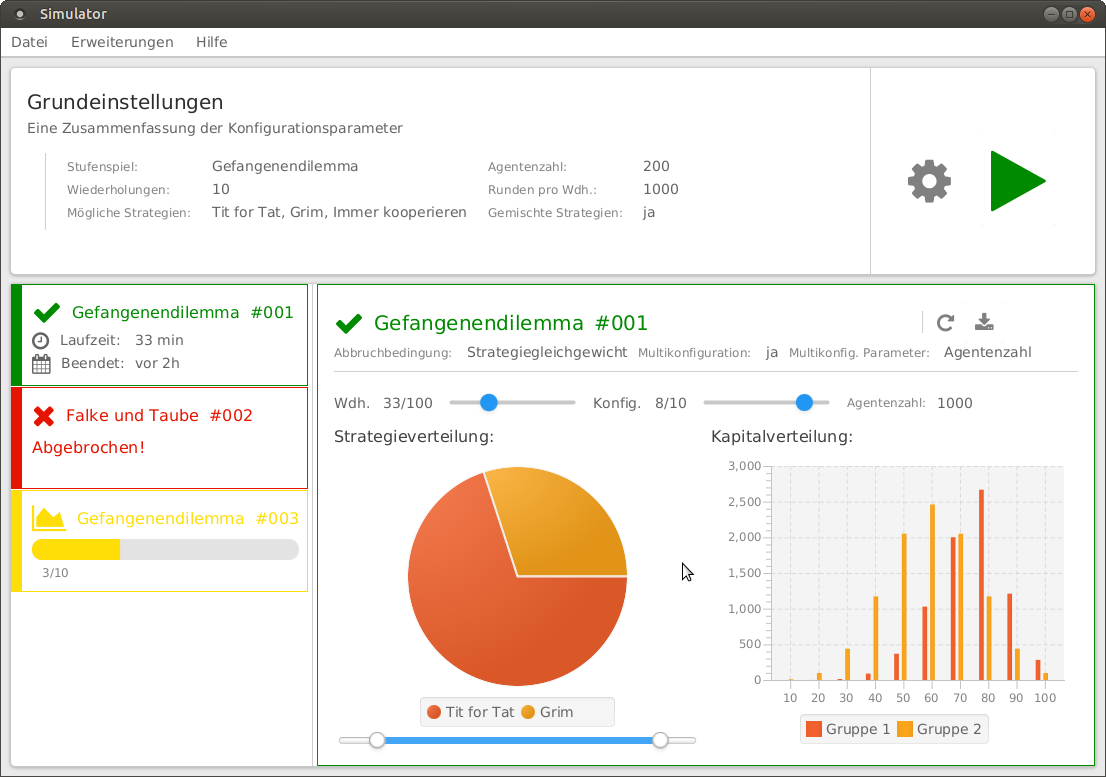
\includegraphics[width=\textwidth]{images/home.png}
	\caption{\label{fig:home}
		Hauptfenster des Simulators}
\end{figure}

Im oberen Drittel des Fensters wird eine Zusammenfassung der aktuell ausgewählten Konfiguration angezeigt (siehe \cref{fig:home_top}). Rechts davon befindet sich ein Knopf zum Bearbeiten der Konfiguration und ein weiterer Knopf zum Starten der Simulation (siehe \cref{fig:main_btn}).
 
\begin{figure}[hb]
	\centering
	
\includegraphics[width=\textwidth]{images/home_top.png}
	\caption{\label{fig:home_top}
	Zusammenfassung der aktuell gewählten Konfiguration}
\end{figure} 
 
\begin{figure}[ht]
	\centering
 	
\includegraphics{images/main_btn.png}
 	\caption{\label{fig:main_btn}
 		Knöpfe zum Konfigurieren und Starten einer Simulation}
\end{figure}


\newpage
Im unteren Teil des Fenster befindet sich links eine Historie der gelaufenen, abgebrochenen und noch laufenden Simulationen (siehe \cref{fig:history}). Wird ein Eintrag angeklickt, erscheint rechts eine Zusammenfassung der Ergebnisse der ausgewählten Simulation (siehe \cref{fig:home_output}). Mit den Knöpfen (siehe \cref{fig:out_btn}) kann die Simulation wiederholt werden und die detailierten Ergebnisse als \(.csv\) Datei exportiert werden. Mit Schiebereglern wird die Wiederholung und im Falle einer Multikonfiguration die Konfiguration ausgewählt, für welche die Ergebnisse angezeigt werden.



\begin{figure}[hb]
	\centering
	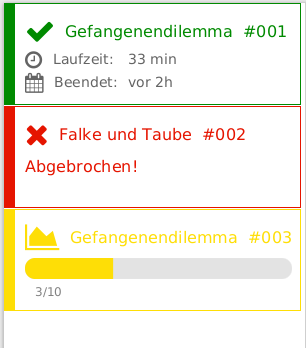
\includegraphics[height=0.5\linewidth ]{images/history.png}
	\caption{\label{fig:history}
		Simulationshistorie }
\end{figure}

\begin{figure}[ht]
	\centering
	
\includegraphics{images/out_btn.png}
	\caption{\label{fig:out_btn}
		Knöpfe zum Wiederholen und Exportieren der Ergebnisse einer Simulation}
\end{figure}
\begin{figure}[ht]
	\centering
	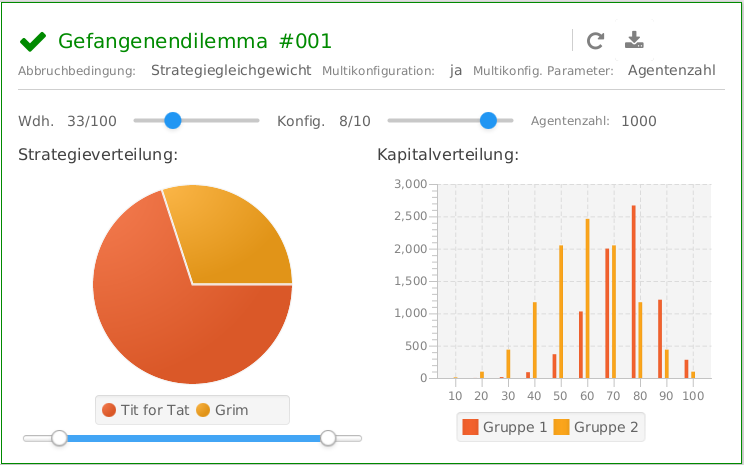
\includegraphics[width=\textwidth]{images/home_output.png}
	\caption{\label{fig:home_output}
		Ausgabe der Ergebnisse einer Simulation}
\end{figure}
\newpage
Über das Dateinmenü in der Menüleiste können Konfigurationen gespeichert und geladen oder eine Simulation gestartet werden (siehe \cref{fig:menu1}).
Das Erweiterungsmenü enthält Optionen zum erstellen eines neuen Stufenspiels oder einer neuen Strategie (siehe \cref{fig:menu2}). Im Hilfemenü finden sich Bedienhilfen und Informationen über den Simulator (siehe \cref{fig:menu3}).

\begin{figure}[ht]
	\centering
	\subfloat[Dateimenü
	\label{fig:menu1}]{%
		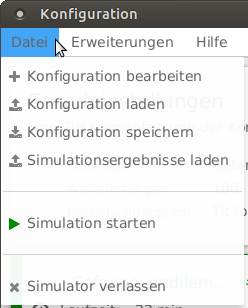
\includegraphics[height=0.25\linewidth]{images/Menu1.png}}
	\qquad
	\subfloat[Erweiterungsmenü
	\label{fig:menu2}]{%
		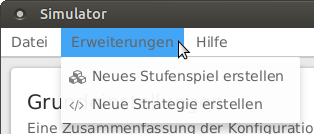
\includegraphics[width=0.25\linewidth]{images/Menu2.png}}
	\qquad
	\subfloat[Hilfemenü
	\label{fig:menu3}]{%
		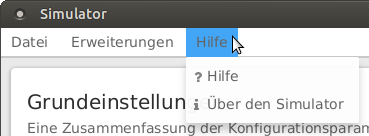
\includegraphics[width=0.25\linewidth]{images/Menu3.png}}
	\caption{\label{fig:menu}
		Funktionen der Menüleiste
	}
\end{figure}
\newpage
Drückt man den Knopf zum Bearbeiten einer Konfiguration, öffnet sich das Konfigurationsfenster (siehe \cref{fig:konfig}).

\begin{figure}[ht]
	\centering
	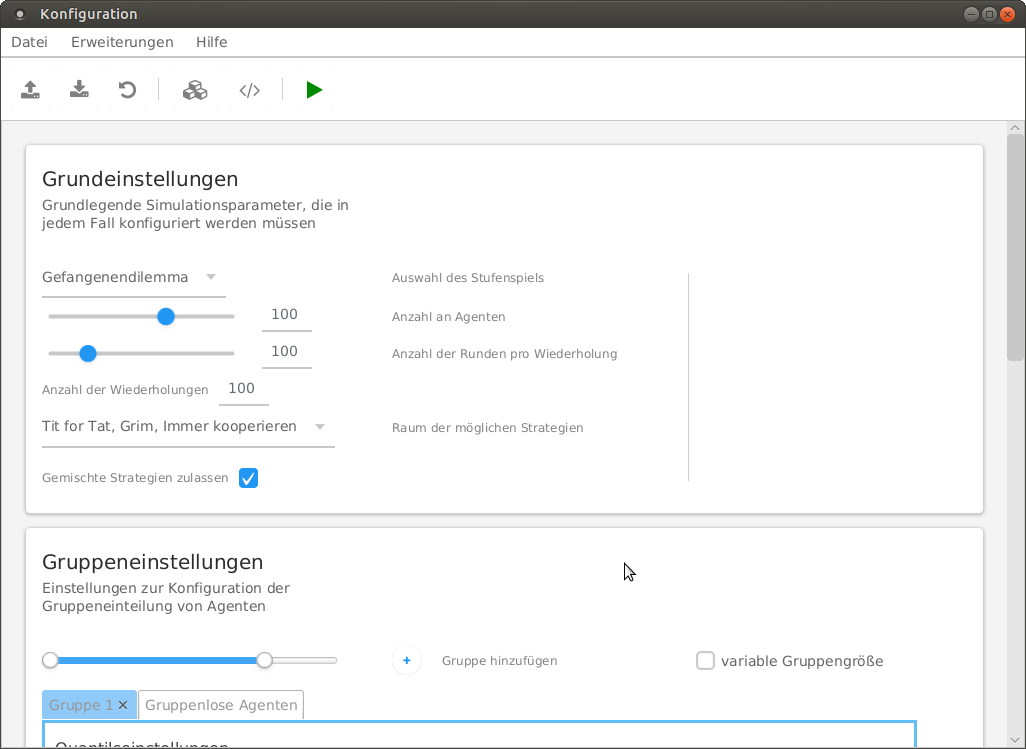
\includegraphics[width=\textwidth]{images/konfig.png}
	\caption{\label{fig:konfig}
		Konfigurationsfenster}
\end{figure} 

Das Konfigrationsfenster ist in drei Bereiche unterteilt, die jeweils ein- und ausgeklappt werden können:
\begin{itemize} \itemsep -10pt
	\item Grundeinstellungen
	\item Gruppeneinstellungen
	\item Erweiterte Einstellungen
\end{itemize}

Grundeinstellungen konfigurieren die fundamentalsten Simulationsparameter (siehe \cref{fig:konfig_main}).

In den Gruppeneinstellungen können Gruppen angelegt und mit einem Multislider die Agenten frei in diese verteilt werden. Für jede Gruppe gibt es einen Tab (siehe \cref{fig:konfig_group}). Dort kann die Gruppe in gleicher Weise weiter in Segmente eingeteilt werden. Für jedes Segment kann das Startkapital der Agenten gemäß einer gewählten Verteilung festgelegt werden (siehe \cref{fig:konfig_cap} und die Initialstrategien eingestellt werden (siehe \cref{fig:konfig_strat}).

\begin{figure}[ht]
	\centering
	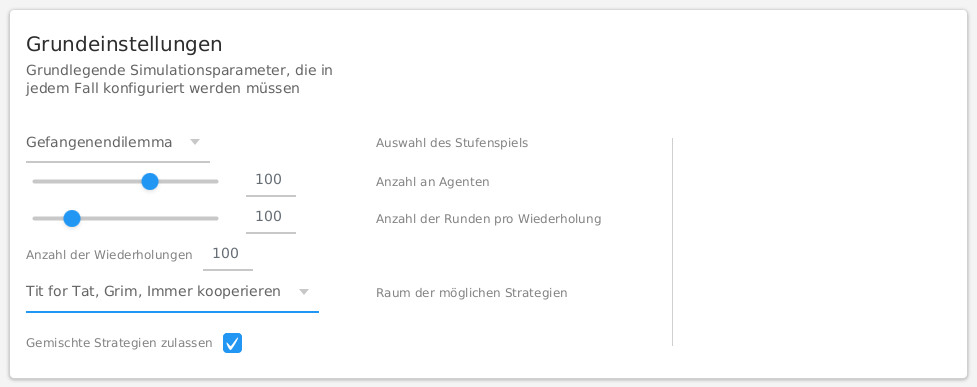
\includegraphics[width=\textwidth]{images/konfig_main.png}
	\caption{\label{fig:konfig_main}
		Grundeinstellungen im Konfigurationsfenster}
\end{figure}

\begin{figure}[ht]
	\centering
	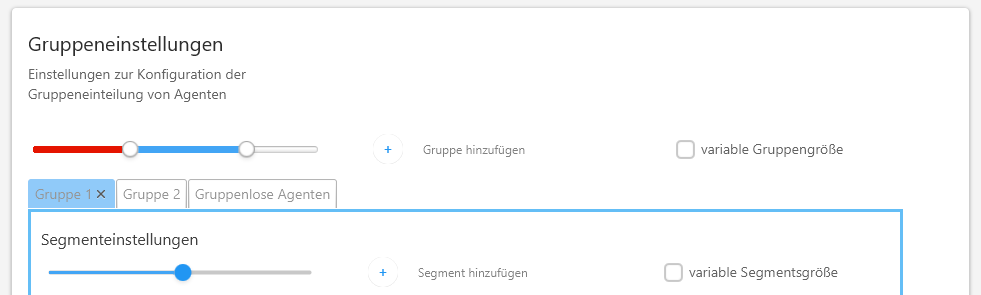
\includegraphics[width=\textwidth]{images/konfig_group.png}
	\caption{\label{fig:konfig_group}
		Gruppeneinstellungen im Konfigurationsfenster}
\end{figure}


In den erweiterten Einstellungen können spezialisierte Konfigurationen per Dropdowns eingestellt werden. Zudem kann hier der variable Konfigurationsparameter eingestellt werden, falls dieser in den Gruppen- bzw. Segementeinstellungen ausgewählt wurde. Dazu wird ein prozentualer Start- und Endwert angegeben und eine Schrittweite festgelegt \\(siehe \cref{fig:konfig_adv}). Hierdurch wird eine Multikonfiguration erstellt.


\newpage
Am oberen Rand des Konfigurationsfenster befindet sich das gleiche Menü wie beim Hauptfenster (siehe \cref{fig:menu} und darunter eine Werkzeugleiste (siehe \cref{fig:konfig_tool}). Über die Werkzeugleiste ist es möglich, Konfigurationen zu laden, zu speichern und die aktuelle Konfiguration auf die Standardwerte zurückzusetzen.\\Darüber hinaus gibt es hier Knöpfe zum Erstellen neuer Stufenspiele und Strategien. Eine Simulation mit der gewählten Konfiguration kann über die Werkzeugleiste gestartet werden.

\begin{figure}[ht]
	\centering
	
\includegraphics[width=\textwidth]{images/konfig_tool.png}
	\caption{\label{fig:konfig_tool}
		Werkzeugleiste des Konfigurationsfenster}
\end{figure}

\begin{figure}[hb]
	\centering
	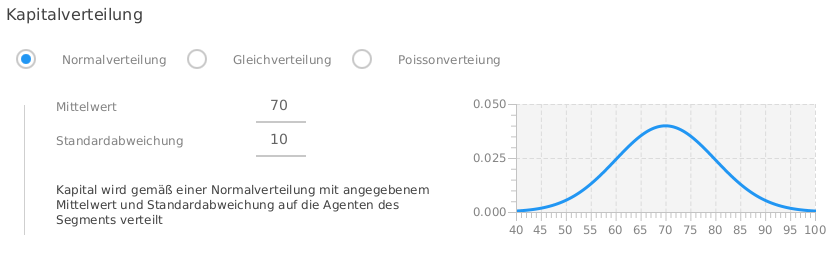
\includegraphics[width=\textwidth]{images/konfig_cap.png}
	\caption{\label{fig:konfig_cap}
		Auswahl der Kapitalverteilung für ein Segment}
\end{figure}

\begin{figure}[hb]
	\centering
	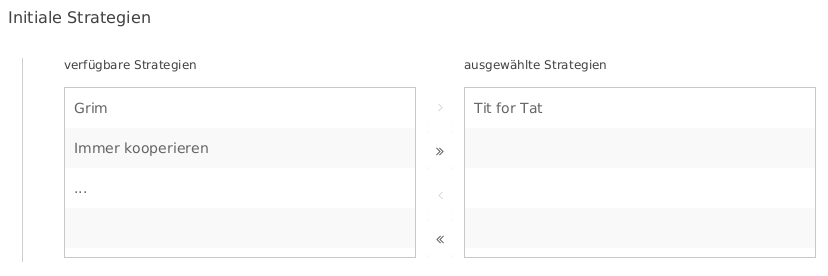
\includegraphics[width=\textwidth]{images/konfig_strat.png}
	\caption{\label{fig:konfig_strat}
		Auswahl der möglichen Initialstrategien für ein Segment}
\end{figure}

\begin{figure}[hb]
	\centering
	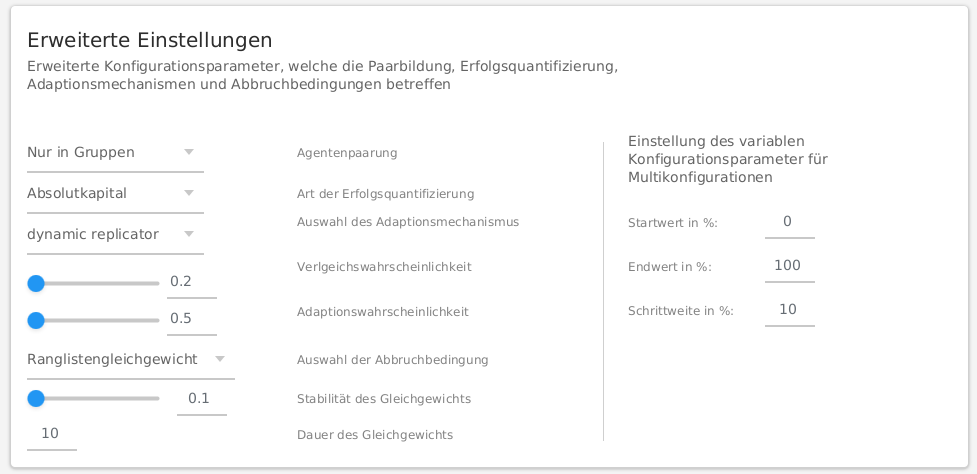
\includegraphics[width=\textwidth]{images/konfig_adv.png}
	\caption{\label{fig:konfig_adv}
		erweiterte Simulationsparameter und Multikonfigurationseinstellungen}
\end{figure}

\newpage

\section{Szenarien}

\subsection{Szenario 1}
Jonas hat die Anwendung auf seinem PC installiert und möchte das Stufenspiel Gefangenendilemma mit 10 Agenten simulieren, wobei von Anfang an eine Hälfte arm und eine Hälfte reich sein soll. Dazu öffnet Jonas die Anwenung und landet im Hauptfenster. Jonas drückt auf das Zahnrad um die von ihm gewünschte Konfiguration einzustellen. Das Konfigurationsfenster öffnet sich und Jonas wählt nun "Gefangenendilemma" bei der Auswahl des Stufenspiel aus und stellt den Slider bei Anzahl der Agenten auf 10. Die Anzahl der Runden und Wiederholungen lässt er auf den voreingestellten Werten. 
Um die Agenten jetzt in 2 Gruppen einzuteilen, erstellt Jonas unter Gruppeneinstellungen 2 neue Gruppen in dem er 2 mal auf das Plus mit "Gruppe hinzufügen" klickt. Er versetzt den Multislider nun so, dass in der einen Gruppe 6 Agenten sind und in der anderen Gruppe 4. Er klickt auf den Bereich des Multislider der an Gruppe 1 zugeteilt wurde und stellt im Unterpunkt Kapitalverteilung eine Normalverteilung mit Mittelwert 200 und Standardabweichung 5 ein. Gleiches tut er für Gruppe 2, jedoch wählt er hier als Mittelpunkt 40. Für beide Gruppen wählt er unter Strategieeinteilung nur "Grim".
Jonas ist zufrieden mit seiner Konfiguration und startet diese nun mit einem Klick auf den grünen Play-Button in der Header-Leiste.
Er wird zurück ins Hauptfesnter navigiert und sieht seine Simulation nun in der Simulations-Historie. Sie ist gelb eingefärbt (Sie läuft noch. Nach einer halben Stunde schaut Jonas noch mal nach, seine Simulation ist jetzt grün eingefärbt (Sie ist beendet). Mit einem Klick auf die Simulation öffnet Jonas die Zusammenfassung für seine Simulation und schaut sich nun die Kapitalverteilung für die einzelnen Gruppen an und wertet sie aus. Jonas ist zufrieden mit seinem Ergebnis und schliesst die Anwendung wieder.
\subsection{Szenario 2}

\newpage
\section{Glossar}

\textbf{Gleichgewicht}:
Ein Gleichgewicht im Simulationsablauf ist erreicht, wenn keiner der Agenten mehr seine Strategie ändert.

\textbf{Stufenspiel:}
Ein spieltheoretisches Spiel, welches sich als Bimatrix darstellen lässt. (z.B. das Gefangenen-Dilemma)

\textbf{Erfolg:}
Der Erfolg eines Agenten in einer Folge von Runden wird aus dessen Kapitalauszahlungen in diesen Runden berechnet. Er ist Konfigurationsparameter der Simulation. Beispiel ist die Summe aller Auszahlungen.

\textbf{Kapital:}
Jedem Agenten wird im Laufe einer Wiederholung eine Zahl zugeordnet, die sich aus dem Initialisierungswert zu Beginn der Wiederholung und der Summe der Auszahlungen aus den Stufenspielen der bisherigen Runden zusammensetzt.

\textbf{Gruppenzugehörigkeit:}
In einer Simulation sind die Agenten in eine feste, wohldefinierte Anzahl von Gruppen partitioniert. Die Strategien der Agenten können auf Gruppenzugehörigkeiten Bezug nehmen. Dabei haben zwei Agenten genau dann dieselbe Gruppenzugehörigkeit, wenn beide Mitglieder in derselben Gruppe sind. Insbesondere müssen beide Mitglied in einer Gruppe sein.

\textbf{Gruppenloser Agent:}
Ein Agent, der keiner Gruppe angehört.

\textbf{Konfiguration:}
Festlegung aller initialen Parameter für einen Simulationslauf.

\textbf{Nutzer:}
Eine Person, welche das Programm nutzt.

\textbf{Multislider:}
Ein Schieberegler mit mehreren möglichen Schiebe-Knöpfen.

\textbf{Slider-Abschnitt:}
Bereich auf dem Slider, der nach rechts und links durch den nächstgelegensten Schiebe-Knopf bzw. den Rand des Sliders begrenzt wird.

\textbf{Ausführungsstatus:}
Der Ausführungsstatus einer Simulation beschreibt, ob die Simulation auf Durchführung wartet, gerade durchgeführt wird oder bereits abgeschlossen ist. 

\textbf{Gemischte Strategie:}
Seien \(S_1,...,S_n\) die in einem Simulationsdurchlauf zugelassenen reinen Strategien. Eine gemischte Strategie ist dann ein Tupel \((\omega_1,...,\omega_n) \in \{0,\frac{1}{10},...,\frac{9}{10},1\}^n\) mit \(\sum_{i=1}^n \omega_i = 1\). \(\omega_i\) entspricht dann der Wahrscheinlichkeit, in einer Runde mit Strategie \(S_i\) zu spielen.

\end{document}
